\documentclass[12pt, a4paper]{report}
\usepackage[utf8]{vietnam}
\usepackage[top=2cm, bottom=1.6cm, left=1.2cm, right=1.5cm]{geometry}
\usepackage{amsmath,amsfonts,amssymb}
\usepackage{indentfirst,enumitem}
\usepackage{graphicx}
\usepackage[font=small,labelfont=bf]{caption}
\usepackage{multicol}
\usepackage{setspace}
\usepackage{hyperref}
\usepackage{listings}
\usepackage{tabularx}
\usepackage{hyperref}
\usepackage{xcolor}
\usepackage{scrextend}
\usepackage{comment}
\usepackage{soul}
\usepackage{tikz,tkz-tab}
\usepackage{float}
\usepackage{tcolorbox}


\renewcommand\thesection{\Roman{section}}
\renewcommand\thesubsection{\arabic{subsection}}
\def\DN{\textbf{\textit{Định nghĩa. }}}

\title{PHƯƠNG PHÁP TÍNH (Numerical Methods)}
\author{Vũ Nhật Huy}

\begin{document}
\onehalfspacing
\maketitle
\newpage
\tableofcontents
\newpage
\chapter{SỐ GẦN ĐÚNG VÀ SAI SỐ}
\section{Những khái niệm cơ bản.}
\DN Độ sai lệch giữa giá trị gần đúng và giá trị chính xác được gọi là sai số.

\DN Số $a$ được gọi là số gần đúng của số chính xác $A$, ký hiệu $a \approx A$ (đọc là $a$ xấp xỉ $A$) nếu $a$ khác $A$ không đáng kể và được dùng thay cho $A$ trong tính toán.

\DN Đại lượng $\Delta = |a - A|$ được gọi là sai số thật sự của số gần đúng $a$. Trong thực tế, do không biết số chính xác $A$, ta ước lượng một đại lượng dương $\Delta_a$ càng bé càng tốt thỏa điều kiện $|A-a|\leq \Delta_a$ được gọi là sai số tuyệt đối của số gần đúng $a$.

\textbf{Chú ý.} Trong thực tế ta sẽ ký hiệu $A = a \pm \Delta_a$.

\DN Sai số tương đối của số gần đúng $a$ so với số chính xác $A$ là đại lượng $\delta_a$ được tính theo công thức $\delta_a = \dfrac{|A-a|}{|A|}$.

\textbf{Chú ý.} Trong nhiều trường hợp, nếu không biết $A$ ta có thể thay thế $\delta_a = \dfrac{\Delta_a}{|a|}\times 100\%$.
\section{Biểu diễn số thập phân.}
\subsection{Chữ số có nghĩa.}
Mọi số thực $a$ có thể được biểu diễn dưới dạng thập phân hữu hạn hoặc vô hạn. 
\[
    a = \pm (\alpha_m \alpha_{m-1}\ldots \alpha_1 \alpha_0 \alpha_{-1} \alpha_{-2}\ldots \alpha_{-n}) = \pm \sum_{k = -n}^{m} \alpha_k 10^k
\]
\[
    \big( m,n \in \mathbb{N},m\geq 0,n\geq 1,\alpha_m \neq 0, \alpha_k \in \{0,1,\ldots,9\} \big)
\]
Ví dụ: $324.59 = 3\times 10^2 + 2\times 10^1 + 4\times 10^0 + 5\times 10^{-1} + 9\times 10^{-2}$\\
Một số viết ở dạng thập phân có thể gồm nhiều chữ số. Ví dụ $20.25$ có $4$ chữ số, $0.03046$ có $6$ chữ số.

\DN Những chữ số có nghĩa của một số là những chữ số của số đó kể từ chữ số khác không đầu tiên tính từ trái sang phải. Ví dụ: Số $20.25$ có $4$ chữ số có nghĩa, số $0.03047$ cũng có $4$ chữ số có nghĩa.

\DN Làm tròn một số thập phân $a$ là bỏ một số các chữ số bên phải $a$ sau dấu chấm thập phân để được một số $\tilde{a}$ ngắn gọn hơn và gần đúng nhất với số $a$. 

\textbf{Quy tắc.} Để làm tròn đến chữ số thứ $k$ sau dấu chấm thập phân, ta xét chữ số thứ $k+1$ sau dấu chấm thập phân là $\alpha_{k+1}$. Nếu $\alpha_{k+1} \geq 5$, ta tăng $\alpha_{k}$ lên 1 đơn vị, còn nếu $\alpha_{k+1} < 5$ ta giữ nguyên chữ số $\alpha_{k}$. Sau đó bỏ phần đuôi từ chữ số $\alpha_{k+1}$ trở đi.\\
Ví dụ: Làm tròn $\pi = 3.1415926535$ đến chữ số thứ $4,3,2$ sau dấu thập phân ta được $3.1416; 3.142;3.14$.

\DN Sai số thực sự của $\tilde{a}$ so với $a$ được gọi là sai số làm tròn. Vậy $\theta_{\tilde{a}} =|a - \tilde{a}|$.\\
Sai số tuyệt đối của $\tilde{a}$ so với $A$ được đánh giá như sau:
\[
    |\tilde{a} - A| = |(\tilde{a} - a) + (a-A)| \leq |\tilde{a}-a| + |a - A| \leq \theta_{\tilde{a}} + \Delta_a = \Delta_{\tilde{a}}
\]
Vì $\theta_{\tilde{a}} \geq 0$ nên $\Delta_{\tilde{a}} \geq \Delta_a$. Do đó sau khi làm tròn sai số tăng lên. Vì vậy, khi tính toán ta tránh làm tròn các phép toán trung gian, chỉ nên làm tròn kết quả cuối cùng.
\subsection{Sự làm tròn số trong bất đẳng thức.}
Trường hợp làm tròn số trong bất đẳng thức, ta sử dụng khái niệm làm tròn lên và làm tròn xuống. Làm tròn lên hay làm tròn xuống cần lưu ý đến chiều bất đẳng thức. Ví dụ: $a<13.9236$ khi làm tròn lên đến 2 chữ số lẻ sau dấu chấm thập phân ta được $a < 13.93$ và $b > 78.6789$ khi làm tròn xuống đến 2 chữ số lẻ sau dấu chấm thập phân ta được $b > 78.67$.
\subsection{Chữ số đáng tin.}
\DN Cho $a \approx A.$ Chữ số $\alpha_k$ trong phép biểu diễn dưới dạng thập phân được gọi là đáng tin nếu $\Delta_a \leq \dfrac{1}{2} \times 10^k$. Trong trường hợp ngược lại, chữ số $\alpha_k$ được gọi là không đáng tin. Ví dụ: Cho số gần đúng $a = 3.7284$ với sai số tuyệt đối là $\Delta_a = 0.0047$ có 3 chữ số đáng tin là $3,7,2$ và 2 chữ số không đáng tin là $8,4$.
\subsection{Cách viết số gần đúng.}
Chúng ta viết số gần đúng $a$ của số chính xác $A$ với sai số tuyệt đối $\Delta_a$ theo quy tắc sau:
\begin{enumerate}
    \item Viết số gần đúng $a$ kèm theo sai số tuyệt đối $\Delta_a$ dưới dạng $a \pm \Delta_a$. Cách này thường được dùng để biểu diễn các kết quả tính toán hoặc phép đo.
    \item Viết số gần đúng theo quy ước: mọi chữ số có nghĩa đều đáng tin. Điều này có nghĩa là sai số tuyệt đối $\Delta_a$ không lớn hơn một nửa đơn vị của chữ số cuối cùng bên phải.
\end{enumerate}
Ví dụ: $a = 23.54$ thì sai số tuyệt đối $\Delta_a \leq \dfrac{1}{2}\times10^{-2} = 0.005,$ trong khi nếu viết $a = 23.5400$ thì sai số tuyệt đối $\Delta_a \leq \dfrac{1}{2}\times10^{-4} = 0.00005$. Cách này thường dùng để trình bày các bảng số.
\section{Công thúc tổng quát của sai số.}
Cho hàm số khả vi liên tục $y=f\left(x_1, x_2, \ldots, x_n\right)$ và giả sử biết sai số tuyệt đối $\Delta_{x_i}$ của các đối số $x_i(i=\overline{1 . . n})$. Gọi $X_i, Y$ và $x_i, y(i=\overline{1 . . n})$ là các giá trị chính xác và các giá trị gần đúng của đối số và hàm số. Khi đó
\[
|Y-y|=\left|f\left(X_1, X_2, \ldots, X_n\right)-f\left(x_1, x_2, \ldots, x_n\right)\right| \leqslant \sum_{i=1}^n\left|\frac{\partial f}{\partial x_i}\right| \cdot\left|X_i-x_i\right| \leqslant \sum_{i=1}^n\left|\frac{\partial f}{\partial x_i}\right| \cdot \Delta_{x_i}
\]
Vậy sai số tuyệt đối của hàm số y là
\[
\begin{aligned}
 \delta_y &=\dfrac{\Delta_y}{|y|}=\frac{\displaystyle\sum_{i=1}^n\left|\dfrac{\partial f}{\partial x_i}\right| \cdot \Delta_{x_i}}{|f|} \\
&=\sum_{i=1}^n\left|\frac{\partial}{\partial x_i} \ln f\left(x_1, x_2, \ldots, x_n\right)\right| \cdot \Delta_{x_i}
\end{aligned}
\]
Ví dụ: Tính sai số tuyệt đối và sai số tương đối của thể tích hình cầu $V=\dfrac{1}{6} \pi d^3$, biết đường kính $d=3.70 \mathrm{~cm} \pm 0.05 \mathrm{~cm}$ và $\pi=3.14 \pm 0.0016$.
Xem $\pi$ và $d$ là những đối số của hàm số $V$, ta có $\dfrac{\partial V}{\partial \pi}=\dfrac{1}{6} d^3=\dfrac{1}{6} \times(3.70)^3$ và $\dfrac{\partial V}{\partial d}=\dfrac{1}{2} \pi d^2=\dfrac{1}{2} \times(3.14) \times(3.70)^2$.

Vậy $\Delta_V=\left|\dfrac{\partial V}{\partial \pi}\right| \cdot \Delta_\pi+\left|\dfrac{\partial V}{\partial d}\right| \cdot \Delta_d=\dfrac{1}{6} \times(3.70)^3 \times$
$0.0016+\dfrac{1}{2} \times(3.14) \times(3.70)^2 \times 0.05=1.0882$

Do đó $V=\dfrac{1}{6} \pi \cdot d^3=26.5084 \mathrm{~cm}^3 \pm 1.0882 \mathrm{~cm}^3$ và
$\delta_V=\dfrac{1.0882}{26.5084}=0.0411$.
\subsection{Sai số của tổng đại số.}    
Xét hàm số $y= \pm x_1 \pm x_2 \pm \ldots \pm x_n$. Khi đó $\left|\dfrac{\partial f}{\partial x_i}\right|=1,(i=\overline{1 . . n})$. Do đó, sai số tuyệt đối của $y$ là $\Delta_y=\Delta_{x_1}+\Delta_{x_2}+\ldots+\Delta_{x_n}$ và sai số tương đối của $y$ là $\delta_y=\dfrac{\Delta_y}{|y|}$.

Ví dụ: Tính sai số tuyệt đối và sai số tương đối của $y=a+b+c$ với $a=47.132 \pm 0.003 ; b=$ $47.111 \pm 0.02 ; c=45.234 \pm 0.5$.
Sai số tuyệt đối của y là $\Delta_y=\Delta_a+\Delta_b+\Delta_c=0.003+0.02+0.5=0.523$.

Do $Y=y \pm \Delta_y=139.477 \pm 0.523$ nên sai số tương đối của $y$ là $\delta_y=\dfrac{\Delta_y}{|y|}=0.0037$.
\subsection{Sai số của tích.}
Xét hàm số $y=x_1 \cdot x_2 \ldots x_n$. Khi đó $\left|\dfrac{\partial}{\partial x_i} \ln y\right|=\dfrac{1}{\left|x_i\right|}, \quad(i=\overline{1 . . n})$. Do đó, sai số tương đối của $y$ là $\delta_y=\delta_{x_1}+\delta_{x_2}+\ldots+\delta_{x_n}$ và sai số tuyệt đối của $y$ là $\Delta_y=\delta_y \cdot|y|$.

Ví dụ: Tính sai số tuyệt đối và sai số tương đối của $y=a . b . c$ với $a=47.132 \pm 0.003 ; b=$ $47.111 \pm 0.02 ; c=45.234 \pm 0.5$. Ta có $\delta_a=\dfrac{\Delta_a}{|a|}, \delta_b=\dfrac{\Delta_b}{|b|}, \delta_c=\dfrac{\Delta_c}{|c|}.$

Sai số tương đối của y là $\delta_y=\delta_a+\delta_b+\delta_c=$ $\dfrac{0.003}{47.132}+\dfrac{0.02}{47.111}+\dfrac{0.5}{45.234}=0.0115$.
Do đó sai số tuyệt đối của y là $\Delta_y=\delta_y \cdot|y|=\left(\dfrac{0.003}{47.132}+\dfrac{0.02}{47.111}+\dfrac{0.5}{45.234}\right) \times$ $(47.132 \times 47.111 \times 4.15 .234)=1159.2503$.
%--------------------------------------------------------------------------------------------------------------------------------------------------------------------------------------------------------------------------------------------------------------------------------------------------------------------------------------------------------------------------------
\chapter{PHƯƠNG TRÌNH PHI TUYẾN}
\section{Khoảng cách ly nghiệm.}
Xét $f(x) = 0 \quad (1)$

\DN Khoảng đóng $\lbrack a,b \rbrack$, hoặc khoảng mở $(a,b)$, mà trên đó tồn tại duy nhất 1 nghiệm của phương trình $(1)$ được gọi là khoảng cách ly nghiệm.

Việc tính nghiệm thực gần đúng của phương trình $(1)$ được tiến hành theo 2 bước:
\begin{enumerate}
    \item Tìm tất cả các khoảng cách ly nghiệm của pt $(1)$.
    \item Trong từng khoảng cách ly nghiệm, tìm nghiệm gần đúng của phương trình bẳng phương pháp nào đó với sai số cho trước.
\end{enumerate}

\textbf{Định lý.} Nếu hàm số $f(x)$ liên tục trong $(a,b)$ và $f(a).f(b)<0$, $f'(x)$ tồn tại và giữ dấu không đổi trong $(a,b)$ thì trong $(a,b)$ chỉ có 1 nghiệm thực duy nhất của phương trình $(1)$.
\begin{center}
    
\includegraphics[scale = 0.38]{1.png}
\end{center}

\textbf{Định lý.} Giả sử hàm $f(x)$ liên tục trên $\lbrack a,b \rbrack$, khả vi trong $(a,b)$. Nếu $x^*$ là nghiệm gần đúng của nghiệm chính xác $\overline{x}$ trong $\lbrack a,b \rbrack$ và $\forall x \in \lbrack a,b \rbrack, |f'(x)| \geq m > 0$ thì công thức đánh giá sai số tổng quát là
\[
    |x^* - \overline{x}| \leq \frac{|f(x^*)|}{m} \Rightarrow m \leq \dfrac{|f(x^*)|}{\min f'(x)} 
\]
\section{Phương pháp chia đôi.}
\begin{center}
    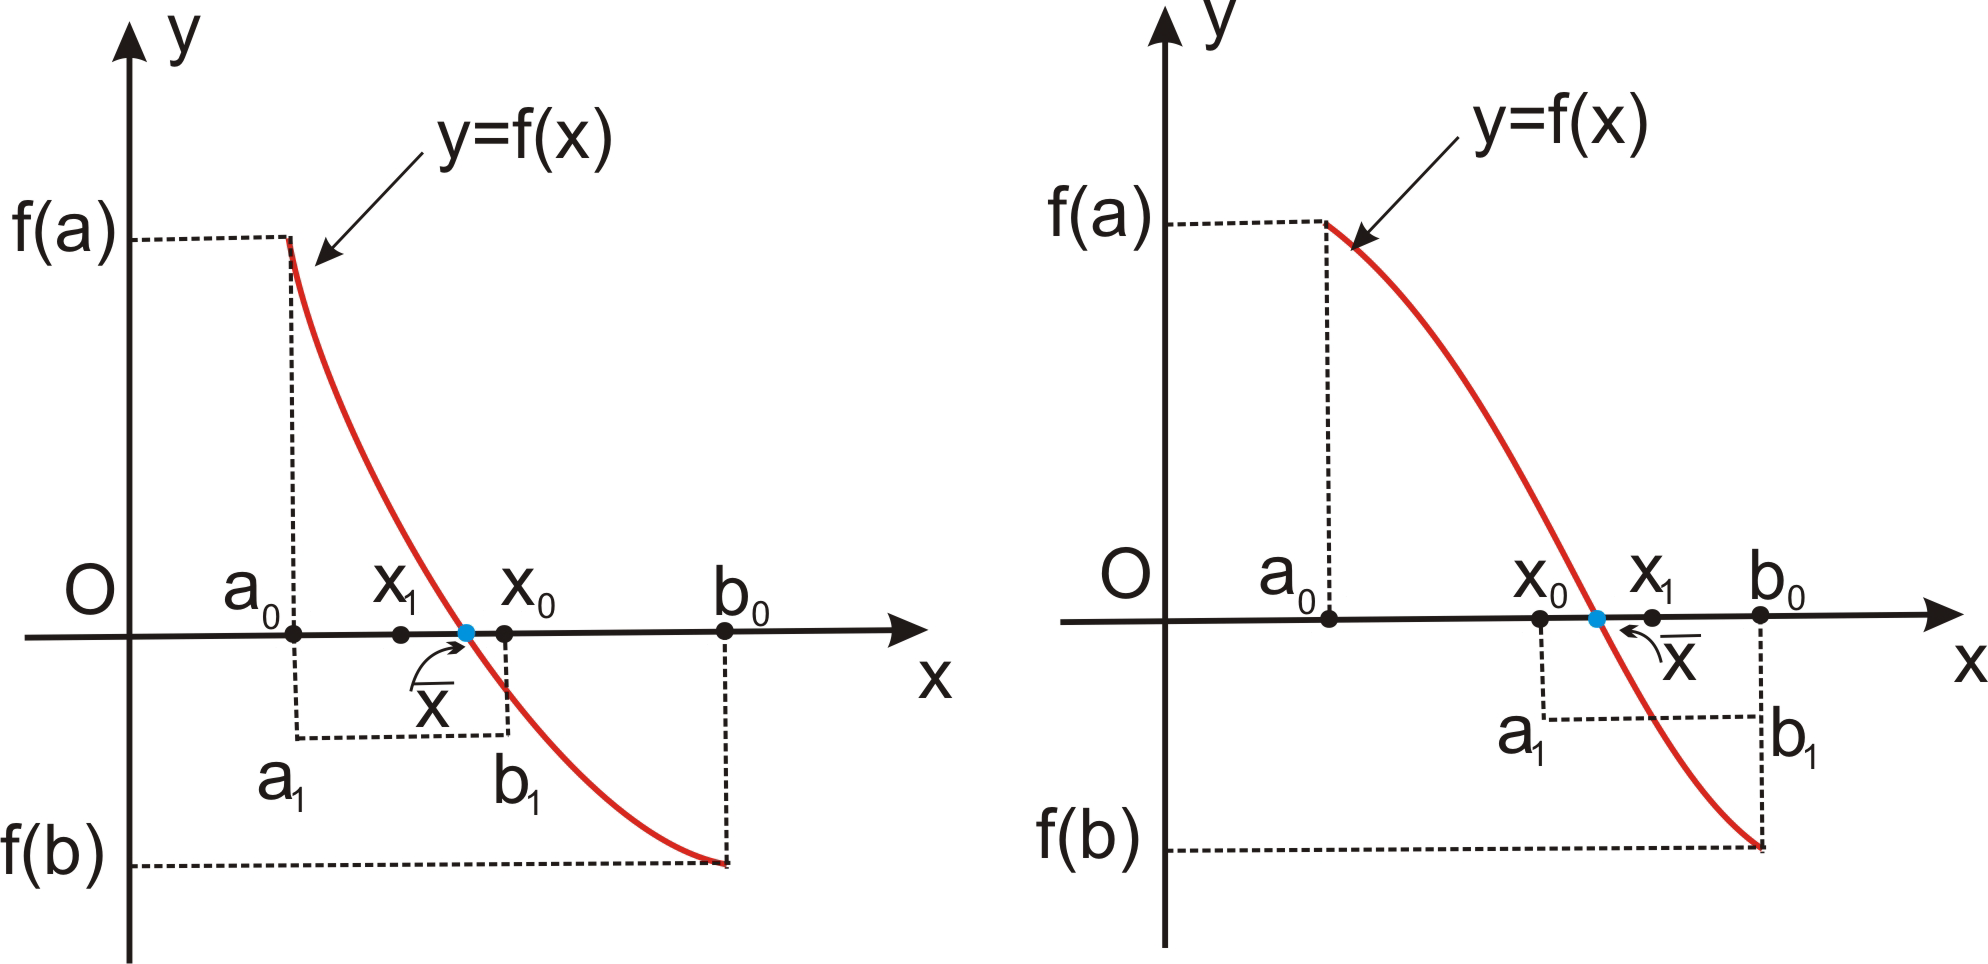
\includegraphics[scale = 0.38]{2.png}
\end{center}
Giả sử $(a,b)$ là khoảng cách ly nghiệm của phương trình $(1)$. Nội dung của phương pháp chia đôi như sau:
\begin{itemize}
    \item Giả sử phương trình $(1)$ có nghiệm chính xác $\overline{x}$ trong khoảng cách ly nghiệm $\lbrack a,b \rbrack$ và $f(a).f(b)<0$. Đặt $a_0 = a, b_0 = b, d_0 = b_0 - a_0 = b - a$ và $x_0 = \dfrac{a_0 + b_0}{2}$ là điểm giữa của đoạn $\lbrack a,b \rbrack$.
    \item Nếu $f(x_0)=0$ thì $x_0$ chính là nghiệm và dừng lại. Ngược lại nếu $f(x_0).f(a_0)<0$ thì dặt $a_1 = a_0,b_1 = x_0$. Nếu $f(x_0).f(b_0)<0$ thì đặt $a_1 = x_0, b_1 = b_0$. Như vậy ta được $\lbrack a,b \rbrack \subset \lbrack a_0,b_0 \rbrack$ và $d_1 = b_1 - a_1 = \dfrac{d_0}{2} = \dfrac{b-a}{2}$.
    \item Tiếp tục quá trình chia đôi đối với $\lbrack a_1,b_1 \rbrack, \lbrack a_2,b_2 \rbrack,\ldots,\lbrack a_{n-1},b_{n-1} \rbrack$ $n$ lần, ta được
\end{itemize}
\[
    \begin{cases}
        a_n \leq \overline{x} \leq b_n, a_n \leq x_n = \dfrac{a_n+b_n}{2}\leq b_n\\
        f(a_n).f(b_n)<0, d_n = b_n - a_n = \dfrac{b-a}{2^n}
    \end{cases}    
\]
Công thức đánh giá sai số.
\[
    |x_n - \overline{x}| = \left\lvert \frac{a_n + b_n}{2}-\overline{x} \right\lvert \leq \frac{1}{2}(b_n - a_n) = \frac{b-a}{2^{n+1}}   
\]
\section{Phương pháp lặp.}
\DN Hàm $g(x)$ được gọi là hàm co trong đoạn $\lbrack a,b \rbrack$ nếu tồn tại số $q \in \lbrack 0,1)$, gọi là hệ số co, sao cho
\[
    \forall x_1,x_2 \in \lbrack a,b \rbrack \Rightarrow |g(x_1) - g(x_2)| \leq q|x_1 - x_2|
\]

\textbf{Định lý.} Nếu $g(x)$ là hàm liên tục trên $\lbrack a,b \rbrack$, khả vi trong $(a,b)$ và $\exists q \in \lbrack0,1)$ sao cho $\forall x \in (a,b), |g'(x)|\leq q$ thì $g(x)$ là hàm co trên $\lbrack a,b \rbrack$ với hệ số co là $q$.

\textbf{Nội dung phương pháp.} Giả sử $\lbrack a,b \rbrack$ là khoảng cách ly nghiệm của phương trình $f(x)=0$. ND của phương pháp lặp là đưa phương trình này về phương trình tương đương $x=g(x)$ sao cho $g(x)$ là hàm co trên $\lbrack a,b \rbrack$. Xây dựng dãy lặp $x_n = g(x_{n-1})$, khi đó với $x_0 \in \lbrack a,b \rbrack$ bất kỳ, dãy lặp sẽ hội tụ về nghiệm của phương trình đã cho.

\textbf{Nguyên lý ánh xạ co.} Giả sử $g(x)$ là hàm co trên đoạn $\lbrack a,b \rbrack$ với hệ số co là $q$. Ngoài ra $g: \lbrack a,b \rbrack \to \lbrack a,b \rbrack$. Khi đó với mọi giá trị $x_0$ ban đầu trong $\lbrack a,b \rbrack$, dãy lặp $(x_n)$ được xác định theo công thức $x_n = g(x_{n-1})$ sẽ họi tụ về nghiệm duy nhất $\overline{x}$ của phương trình $x=g(x)$ và ta có công thức đánh giá sai số:
\[
    \begin{aligned}
        &|x_n - \overline{x}| \leq \dfrac{q^n}{1-q}|x_1 - x_0|: \text{tiên nghiệm}\\
        &|x_n - \overline{x}| \leq \dfrac{q}{1-q}|x_n - x_{n-1}|: \text{hậu nghiệm}
    \end{aligned}    
\]
\begin{center}
    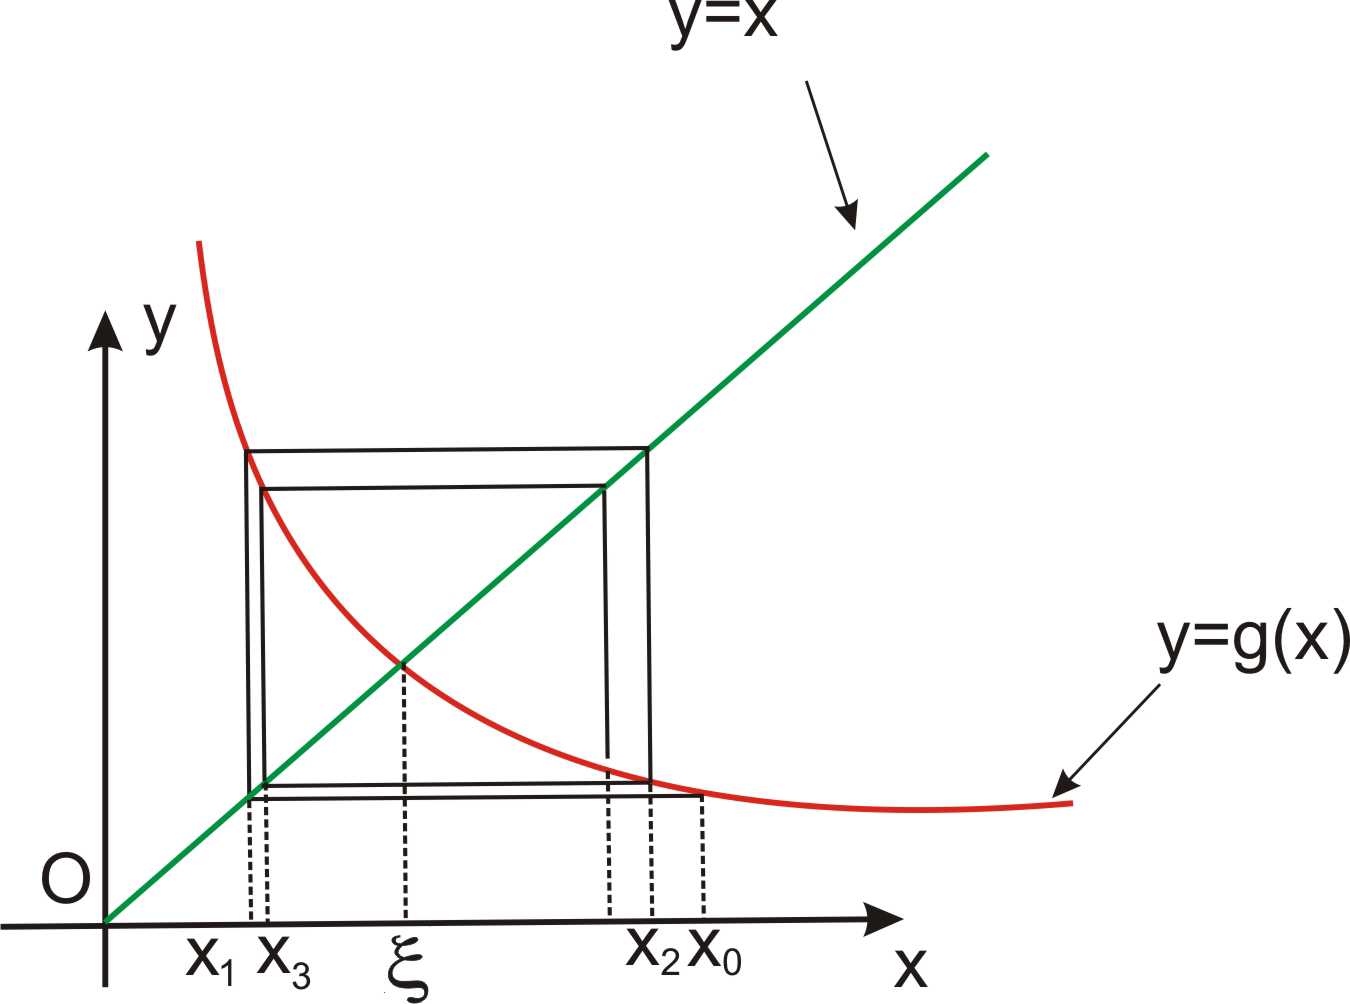
\includegraphics[scale = 0.38]{3.png}
\end{center}
Chú ý. Sự hội tụ của phương pháp lặp càng nhanh nêu $q$ càng bé.
\section{Phương pháp Newton.}
Cho phương trình $f(x) = 0, x \in (a,b)$. \\
Gọi $x^*$ là nghiệm gần đúng, $\overline{x}$ là nghiệm chính xác. Áp dụng công thức Taylor:
\[
    \begin{aligned}
        & f(\overline{x}) = f(x^*) + f'(x^*)(\overline{x}-x^*) + o(\overline{x}-x^*)\\
        & \longrightarrow 0 = f(\overline{x}) \approx f(x^*) + f'(x^*)(\overline{x}-x^*)\\
        & \overline{x} \approx x^* - \dfrac{f(x^*)}{f'(x^*)}
    \end{aligned}    
\]
Xây dựng dãy lặp Newton: $x_n = x_{n-1} - \dfrac{f(x_{n-1})}{f'(x_{n-1})}$. Từ công thức Newton suy ra: 
\[
    0 - f(x_{n-1}) = f'(x_{n-1})(x_n - x_{n-1})
\]
Từ đây ta có thể suy ra cách xác định $x_n$ từ $x_{n-1}$ như sau: từ điểm $(x_{n-1},f(x_{n-1}))$ trên đồ thị, ta vẽ tiếp tuyến với đồ thị tại điểm này, $x_{n}$ là giao điểm của tiếp tuyến này với trục hoành. Phương pháp Newton còn gọi là phương pháp tiếp tuyến.
\begin{center}
    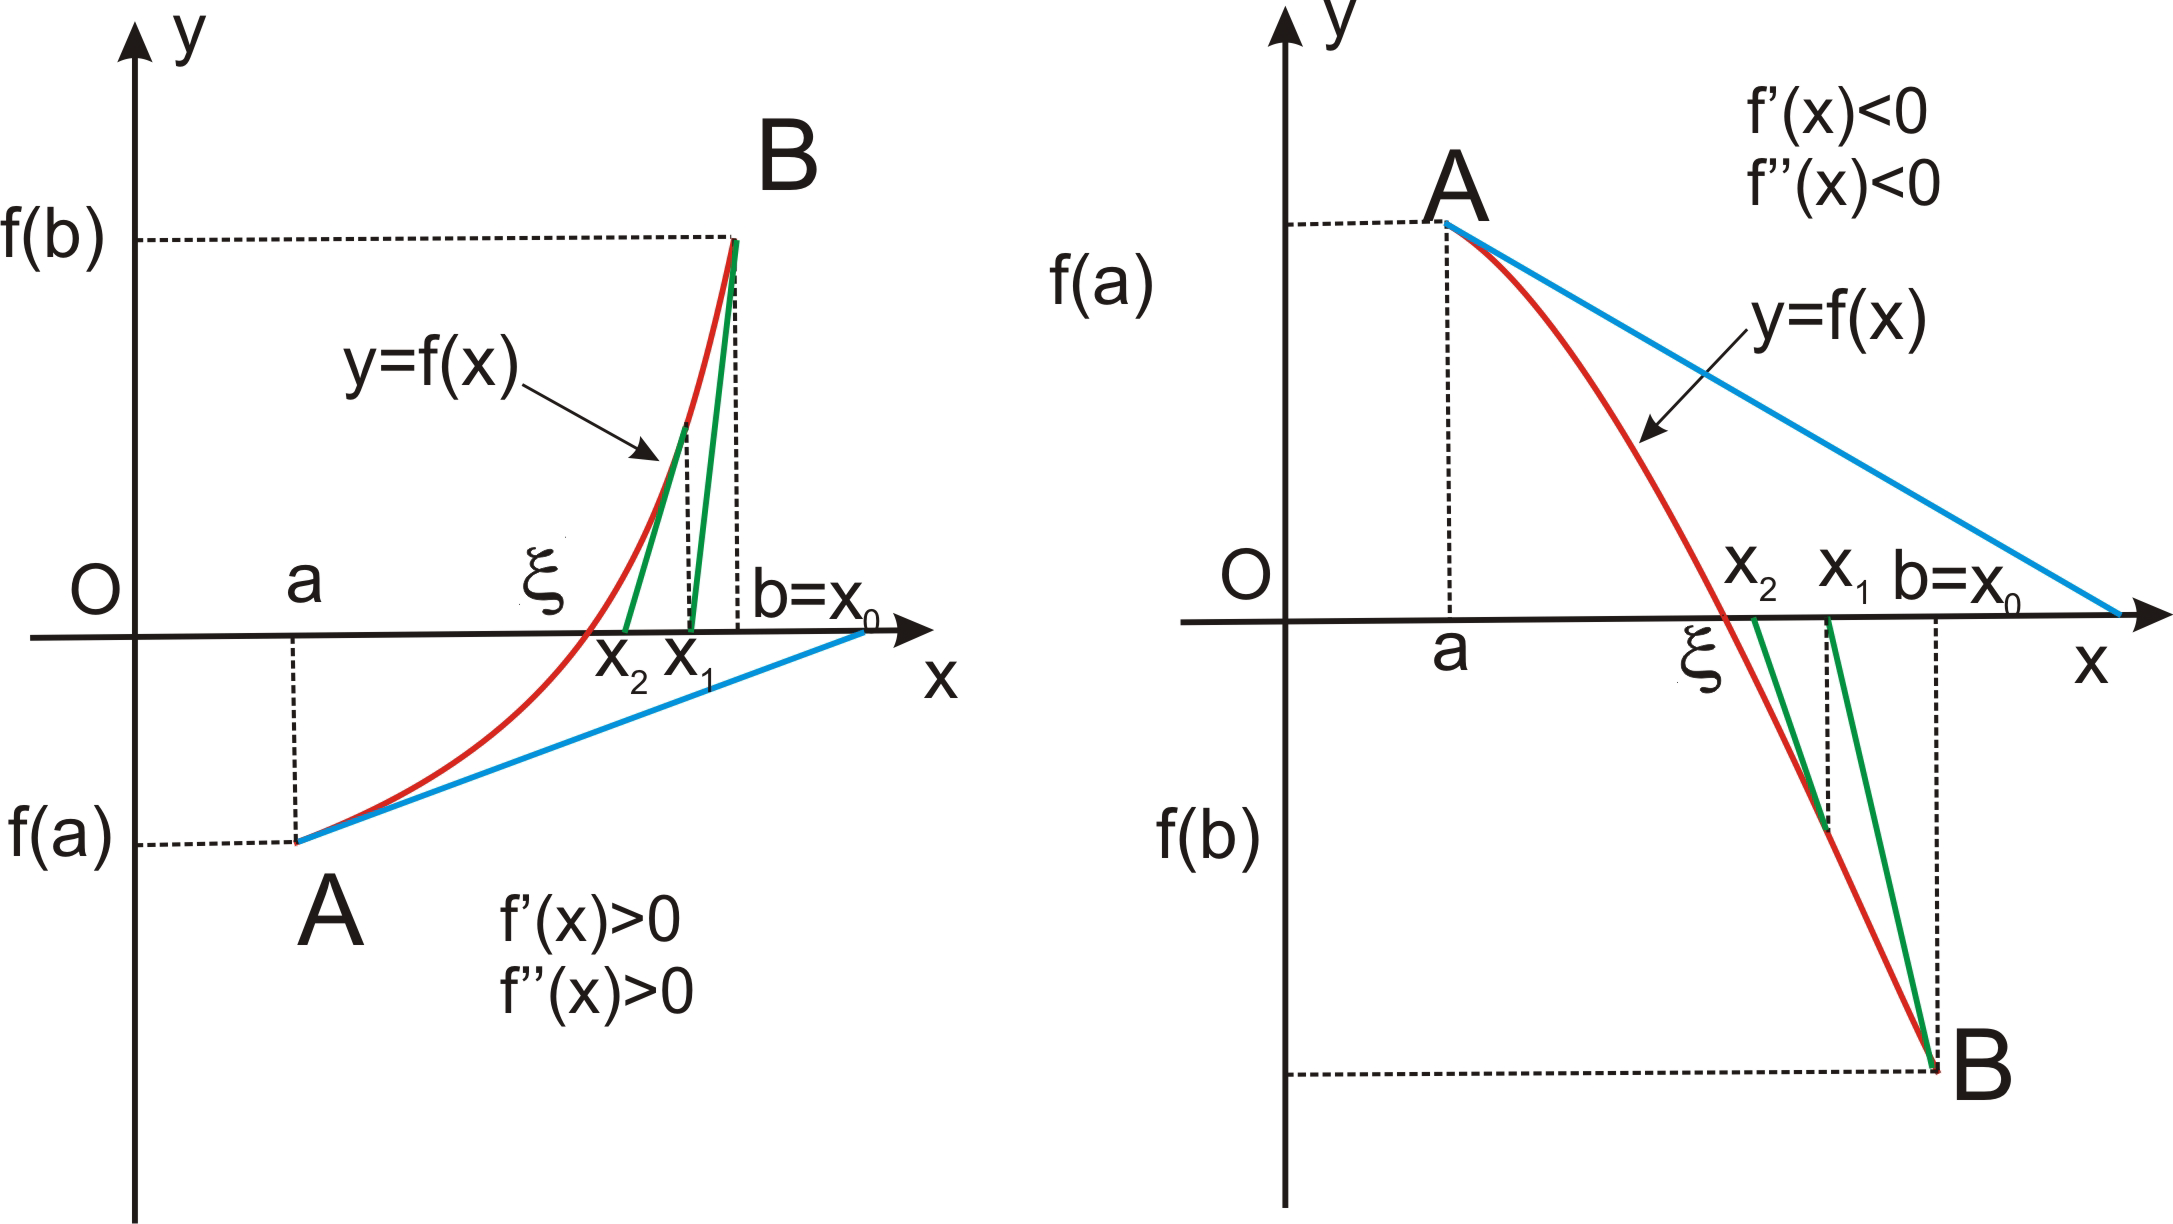
\includegraphics[scale = 0.35]{4.png}
\end{center}
Công thức sai số tổng quát của phương pháp Newton:
\[
    \Delta x_n = |x_n - \overline{x}| \leq \frac{f(x_n)}{\displaystyle\min_{x \in \lbrack a,b \rbrack} |f'(x)|}    
\]
Nếu xem phương pháp Newton như lặp đơn, khi đó: 
\[
    g(x) = x - \frac{f(x)}{f'(x)} 
\]
Nhận thấy $g'(\overline{x}) = 0$, nếu chọn $x_0$ thích hợp thì phương pháp Newton sẽ hội tụ nhanh (nhờ hệ số co nhỏ), nhưng nếu chọn $x_0$ không phù hợp phương pháp Newton có thể không hội tụ $(g'(x)>1)$.
%\begin{mytheo}{This is my title}
%    This is the text of the theorem. The counter is automatically assigned and,
%    in this example, prefixed with the section number. This theorem is numbered with
%     and is given on page.
%  \end{mytheo}
\newpage
\chapter{HỆ PHƯƠNG TRÌNH TUYẾN TÍNH}
\section{Phương pháp nhân tử LU.}
\subsection{Những khái niệm cơ bản.}
Ma trận vuông $\begin{pmatrix}
    a_{11} & a_{12} &  \dots  & a_{1n} \\
    0 & a_{22} &  \dots  & a_{2n} \\
    \vdots & \vdots & \ddots & \vdots\\
    0 & 0 &  \dots  & a_{nn}
\end{pmatrix}$ được gọi là ma trận tam giác trên. 

Ma trận vuông $\begin{pmatrix}
    a_{11} & 0 & 0  & 0 \\
    a_{21} & a_{22} & \dots  & 0 \\
    \vdots & \vdots & \ddots & \vdots \\
    a_{n1} & a_{n2} & \dots  & a_{nn}
\end{pmatrix}$ được gọi là ma trận tam giác dưới.
\subsection{Nội dung phương pháp.}
Phân tích ma trận $A$ thành tích 2 ma trận $L$ và $U$, trong đó $L$ là ma trận tam giác dưới, còn $U$ là ma trận tam giác trên. Khi đó việc giải hệ phương trình tuyến tính sẽ trờ thành giải 2 hệ phương trình $LY=B$ và $UX = Y$. Ta sẽ phân tích theo phương pháp Doolittle. Khi đó $L$ và $U$ sẽ có dạng:
\[
    L = \begin{pmatrix}
        1 & 0 & 0  & 0 \\
        l_{21} & 1 & \dots  & 0 \\
        \vdots & \vdots & \ddots & \vdots \\
        l_{n1} & l_{n2} & \dots  & 1
    \end{pmatrix} \qquad U = \begin{pmatrix}
        u_{11} & u_{12} &  \dots  & u_{1n} \\
        0 & u_{22} &  \dots  & u_{2n} \\
        \vdots & \vdots & \ddots & \vdots\\
        0 & 0 &  \dots  & u_{nn}
    \end{pmatrix}
\]
Các phần tử của 2 ma trận $L$ và $U$ được xác định theo công thức
\[
    \begin{cases}
        u_{1j} = a_{1j} \qquad (1 \leq j \leq n) \\
        l_{i1} = \dfrac{a_{i1}}{u_{11}} \qquad (2 \leq i \leq n) \\
        u_{ij} = a_{ij} - \displaystyle \sum_{k=1}^{i-1} l_{ik}.u_{kj} \qquad (1 < i \leq j) \\
        l_{ij} = \dfrac{1}{u_{ij}} \left( \displaystyle a_{ij} \sum_{k=1}^{i-1} l_{ik}.u_{kj} \right) \qquad (1<j<i)
    \end{cases}    
\]
Ta có công thức nhanh từ công thức trên đối với ma trận cấp vuông cấp 3 và 4 như sau:
\subsubsection{Ma trận vuông cấp 3.}
\[
    \begin{pmatrix}
        a_{11} & a_{12} & a_{13} \\
        a_{21} & a_{22} & a_{23} \\
        a_{31} & a_{32} & a_{33} \\
    \end{pmatrix}  = \begin{pmatrix}
        1 & 0 & 0 \\
        \textcolor{red}{l_{21}} & 1 & 0 \\
        \textcolor{red}{l_{31}} & \textcolor{red}{l_{32}} & 1 \\
    \end{pmatrix} \begin{pmatrix}
        \textcolor{red}{u_{11}} & \textcolor{red}{u_{12}} & \textcolor{red}{u_{13}} \\
        0 & \textcolor{red}{u_{22}} & \textcolor{red}{u_{23}} \\
        0 & 0 & \textcolor{red}{u_{33}} \\
    \end{pmatrix}
\]
\[
    \begin{pmatrix}
        a_{11} & a_{12} & a_{13} \\
        a_{21} & a_{22} & a_{23} \\
        a_{31} & a_{32} & a_{33} \\
    \end{pmatrix}  = \begin{pmatrix}
        1 & 0 & 0 \\
        \textcolor{red}{a_{21}/a_{11}} & 1 & 0 \\
        \textcolor{red}{a_{31}/a_{11}} & \textcolor{blue}{l_{32}}  & 1 \\
    \end{pmatrix} \begin{pmatrix}
        \textcolor{red}{a_{11}} & \textcolor{red}{a_{12}} & \textcolor{red}{a_{13}} \\
        0 & \textcolor{red}{D_2/D_1} & \textcolor{blue}{u_{23}} \\
        0 & 0 & \textcolor{red}{D_3/D_2} \\
    \end{pmatrix}
\]
\[
    d_3 \times c_2 \Rightarrow \frac{a_{31}.a_{12}}{a_{11}} +  \textcolor{blue}{l_{32}}.\dfrac{D_2}{D_1} = a_{32}; \thickspace d_2 \times c_3 \Rightarrow \frac{a_{21}.a_{13}}{a_{11}}+ \textcolor{blue}{u_{23}}=a_{23}
\]
\subsubsection{Ma trận vuông cấp 4.}
\[
    \begin{pmatrix}
        a_{11} & a_{12} & a_{13} & a_{14}\\
        a_{21} & a_{22} & a_{23} & a_{24}\\
        a_{31} & a_{32} & a_{33} & a_{34}\\
        a_{41} & a_{42} & a_{43} & a_{44}\\
    \end{pmatrix}  = \begin{pmatrix}
        1 & 0 & 0 & 0\\
        \textcolor{red}{a_{21}/a_{11}} & 1 & 0 & 0\\
        \textcolor{red}{a_{31}/a_{11}} & \textcolor{blue}{l_{32}} & 1 & 0\\
        \textcolor{red}{a_{41}/a_{11}} & \textcolor{blue}{l_{42}} & \textcolor{blue}{l_{43}} & 1
    \end{pmatrix} \begin{pmatrix}
        \textcolor{red}{a_{11}} & \textcolor{red}{a_{12}} & \textcolor{red}{a_{13}} & \textcolor{red}{a_{14}}\\
        0 & \textcolor{red}{D_2/D_1} & \textcolor{blue}{u_{23}} & \textcolor{blue}{u_{24}}\\
        0 & 0 & \textcolor{red}{D_3/D_2} & \textcolor{blue}{u_{34}} \\
        0 & 0 & 0 & \textcolor{red}{D_4/D_3}
    \end{pmatrix}
\]
\[
    d_3 \times c_2 \Rightarrow \frac{a_{31}.a_{12}}{a_{11}} +  \textcolor{blue}{l_{32}}.\dfrac{D_2}{D_1} = a_{32}; \thickspace d_2 \times c_3 \Rightarrow \frac{a_{21}.a_{13}}{a_{11}}+ \textcolor{blue}{u_{23}}=a_{23}
\]
\[
    d_4 \times c_2 \Rightarrow \frac{a_{41}.a_{12}}{a_{11}} +  \textcolor{blue}{l_{42}}.\dfrac{D_2}{D_1} = a_{42}; \thickspace d_2 \times c_4 \Rightarrow \frac{a_{21}.a_{14}}{a_{11}}+ \textcolor{blue}{u_{24}}=a_{24}
\]
\[
    d_4 \times c_3 \Rightarrow \frac{a_{41}.a_{13}}{a_{11}} + \textcolor{magenta}{l_{42}.u_{23}} + \textcolor{blue}{l_{43}}.\dfrac{D_3}{D_2} = a_{43}; \thickspace d_3 \times c_4 \Rightarrow \frac{a_{31}.a_{14}}{a_{11}}+ \textcolor{magenta}{l_{32}.u_{24}} + \textcolor{blue}{u_{34}}=a_{34}
\]
\newpage
\section{Phương pháp Choleski.}
Một ma trận vuông A đối xứng và xác định dương có thể phân tích duy nhất được dưới dạng $A=B.B^T$, với B là ma trận tam giác dưới. Ma trận vuông A xác định dương nếu các định thức con chính của nó đều dương.
\[
    \begin{pmatrix}
        a_{11} & a_{12} &  \dots  & a_{1n} \\
        a_{21} & a_{22} &  \dots  & a_{2n} \\
        \vdots & \vdots & \ddots & \vdots\\
        a_{n1} & a_{n2} &  \dots  & a_{nn}
    \end{pmatrix} = \begin{pmatrix}
        B_{11} & 0 & 0  & 0 \\
        B_{21} & B_{22} & \dots  & 0 \\
        \vdots & \vdots & \ddots & \vdots \\
        B_{n1} & B_{n2} & \dots  & B_{nn}
    \end{pmatrix} \begin{pmatrix}
        B_{11} & B_{12} &  \dots  & B_{1n} \\
        0 & a_{22} &  \dots  & B_{2n} \\
        \vdots & \vdots & \ddots & \vdots\\
        0 & 0 &  \dots  & B_{nn}
    \end{pmatrix}
\]
Các phần tử của ma trận B được xác định theo công thức:
\[
    \begin{cases}
        B_{11} = \sqrt{a_{11}} \\
        B_{i1} = \dfrac{a_{i1}}{B_{11}} \qquad (2 \leq i \leq n) \\
        B_{ii} = \sqrt{a_{ii} - \displaystyle \sum_{k=1}^{i-1} B^2_{ik}} \qquad (1 < i \leq n) \\
        B_{ij} = \dfrac{1}{B_{jj}} \left( a_{ij} - \displaystyle \sum_{k=1}^{j-1} B_{ik}.B_{jk} \right) \qquad (1<j<i)
    \end{cases}    
\]
Từ đây ta có công thức nhanh sau:
\[
    \begin{pmatrix}
        a_{11} & a_{12} & a_{13} \\
        a_{21} & a_{22} & a_{23} \\
        a_{31} & a_{32} & a_{33} \\
    \end{pmatrix}  = \begin{pmatrix}
        \textcolor{red}{B_{11}} & 0 & 0 \\
        \textcolor{red}{B_{21}} & \textcolor{red}{B_{22}} & 0 \\
        \textcolor{red}{B_{31}} & \textcolor{red}{B_{32}} & \textcolor{red}{B_{33}} \\
    \end{pmatrix} \begin{pmatrix}
        \textcolor{red}{B_{11}} & \textcolor{red}{B_{12}} & \textcolor{red}{B_{13}} \\
        0 & \textcolor{red}{B_{22}} & \textcolor{red}{B_{23}} \\
        0 & 0 & \textcolor{red}{B_{33}} \\
    \end{pmatrix}    
\]
\[
    \Rightarrow B = \begin{pmatrix}
        \textcolor{red}{\sqrt{D_1}} & 0 & 0 \\
        \textcolor{red}{\dfrac{\textcolor{red}{a_{21}}}{\textcolor{red}{B_{11}}}} & \textcolor{red}{\sqrt{\dfrac{D_2}{D_1}}} & 0 \\
        \textcolor{red}{\dfrac{\textcolor{red}{a_{31}}}{\textcolor{red}{B_{11}}}} & \textcolor{red}{\dfrac{\textcolor{red}{a_{32} - B_{31}.B_{21}}}{\textcolor{red}{B_{22}}}} & \textcolor{red}{\sqrt{\dfrac{D_3}{D_2}}}
    \end{pmatrix}    
\]
\section{Chuẩn của vector, chuẩn của ma trận.}
\subsection{Chuẩn của vector.}
Trong không gian tuyến tính thực $\mathbb{R}^n$. Chuẩn của vector $X \in \mathbb{R}^n$ là một số thực, ký hiệu $||X||$ thỏa
\begin{enumerate}
    \item $\forall X \in \mathbb{R}^n, ||X|| \geq 0, ||X|| = 0 \Leftrightarrow X = 0$ 
    \item $\forall X \in \mathbb{R}^n, \forall \lambda \in \mathbb{R}^n, ||\lambda X|| = |\lambda|.||X||$
    \item $\forall X,Y \in \mathbb{R}^n, ||X+Y|| \leq ||X|| + ||Y||$
\end{enumerate}
Ta thường xét 2 chuẩn sau: $\forall X = (x_1,x_2,\cdots,x_n)^T \in \mathbb{R}^n$
    \begin{enumerate}
        \item $||X||_1 = |x_1|+ |x_2| + \ddots + |x_n| = \displaystyle \sum_{k=1}^{n} |x_k|$
        \item $||X||_{\infty} = \max \lbrace |x_1|,|x_2|,\ddots,|x_n| \rbrace = \max_{k=\overline{1,n}} |x_k|$
    \end{enumerate}    
\subsection{Chuẩn của ma trận.}
Chuẩn của ma trận $A=(a_{ij})$ được xác định như sau:
\begin{itemize}
    \item $||A||_1 = \displaystyle \max_{1\leq j \leq n} \sum_{i=1}^{n} |a_{ij}| \qquad \text{chuẩn cột}$
    \item $||A||_{\infty} = \displaystyle \max_{1\leq i \leq n} \sum_{j=1}^{n} |a_{ij}| \qquad \text{chuẩn hàng}$
\end{itemize}
\section{Những phương pháp lặp.}
Số $k(A)=Cond(A)=||A||.||A^{-1}||$ được gọi là số điều kiện của ma trận A. Số điều kiện $k(A)$ thỏa $1\leq k(A) \leq +\infty$.
\begin{itemize}
    \item $Cond(A)$ gần với 1: Hệ ổn định.
    \item $Cond(A)$ càng lớn: Hệ càng không ổn định.
\end{itemize}
%                           NOTE
%Khúc này có thể ghi AX=b được X=BX+b như vid https://youtu.be/k4e3nJD8GdU?si=EE1xh9uJWnAI7eow&t=2110
Từ hệ $A X=b$, ta phân tích $A=M-N$, với $M$ là ma trận "dễ" khả nghịch, khi đó ta có:
\[
    \begin{aligned}
        & (M-N) X=b \Leftrightarrow M X=N X+b \\
        & \Leftrightarrow X=M^{-1} N X+M^{-1} b
    \end{aligned}
\]
Đặt $T=M^{-1} N, c=M^{-1} b \rightarrow X=T X+c$.\\
Xuất phát từ véctơ ban dầu $X^{(0)}$ ta xây dựng dãy $\left(X^{(m)}\right)_{m=0}^{\infty}$ theo công thức
\[
    X^{(m)}=T X^{(m-1)}+c, \quad m=1,2, \ldots
\]
\textbf{Định lý}. Nếu $\|T\|<1$ thì dãy các véctơ $\left(X^{(m)}\right)_{m=0}^{\infty}$ xác dịnh theo công thức lặp sẽ hội tụ về vécto nghiệm $\bar{X}$ của hệ với mọi véctơ lặp ban đầu $X^{(0)}$. Khi đó công thức đánh giá sai số như sau:
\[
    \left\|X^{(m)}-\bar{X}\right\| \leqslant \frac{\|T\|^m}{1-\|T\|} \cdot\left\|X^{(1)}-X^{(0)}\right\|
\]
hoặc
\[
    \left\|X^{(m)}-\bar{X}\right\| \leqslant \frac{\|T\|}{1-\|T\|} \cdot\left\|X^{(m)}-X^{(m-1)}\right\|
\]
\newpage
\subsection{Phương pháp lặp Jacobi.}
Ma trận A được gọi là ma trận đường chéo trội nhgiêm ngặt nếu như thỏa mãn điều kiện sau đây:
\[
    \displaystyle \sum_{j=1, j \neq i}^{n} | a_{ij} | < | a_{ii} |   
\]
Xét hệ phương trình $AX=b$. Phân tích ma trận A theo dạng:
\[
    \begin{pmatrix}
        a_{11} & a_{12} &  \dots  & a_{1n} \\
        a_{21} & a_{22} &  \dots  & a_{2n} \\
        \dots & \dots &  \dots & \dots\\
        a_{n1} & a_{n2} &  \dots  & a_{nn}
    \end{pmatrix} = \begin{pmatrix}
        a_{11} & 0 &  \dots  & 0 \\
        0 & a_{22} &  \dots  & 0 \\
        \dots & \dots &  \dots & \dots\\
        0 & 0 &  \dots  & a_{nn}
    \end{pmatrix} - \begin{pmatrix}
        0 & 0 &  \dots  & 0 \\
        -a_{21} & 0 &  \dots  & 0 \\
        \dots & \dots &  \dots & \dots\\
        -a_{n1} & -a_{n2} &  \dots  & 0
    \end{pmatrix} - \begin{pmatrix}
        0 & -a_{12} &  \dots  & -a_{1n} \\
        0 & 0 &  \dots  & -a_{2n} \\
        \dots & \dots &  \dots & \dots\\
        0 & 0 &  \dots  & 0
    \end{pmatrix}
\]
\[
    = D - L - U    
\]
Do $a_{ii} \neq 0, \forall i=1,2,\cdots,n$ nên $\det D \neq 0$. Như vậy
\[
    D^{-1} = \begin{pmatrix}
        \dfrac{1}{a_{11}} & 0 &  \dots  & 0 \\
        0 & \dfrac{1}{a_{22}} &  \dots  & 0 \\
        \dots & \dots &  \dots & \dots\\
        0 & 0 &  \dots  & \dfrac{1}{a_{nn}}
    \end{pmatrix}
\]
Khi đó hệ
\[
    AX=b \Longleftrightarrow (D-L-U)X = b \Longleftrightarrow X = D^{-1}(L+U)X + D^{-1}b
\]
Ký hiệu $T_j = D^{-1}(L+U) $ và $c_j = D^{-1}b$. Ta thu được:
\[
    X^{(m)} = T_j X^{(m-1)} + c_j, \qquad m=1,2,3,\cdots
\]
\begin{tcolorbox}[title=Dạng tường minh của công thức lặp Jacobi, titlebox=visible, colframe=red!75!black,colback=red!5!white,fonttitle=\bfseries]
    \[
        x^{(m)}_i = \dfrac{1}{a_{ii}} \left(  -\displaystyle \sum_{j=1}^{i-1}a_{ij}x^{(m-1)}_j - \displaystyle \sum_{j=i+1}^{n}a_{ij}x^{(m-1)}_j + b_i \right)
    \]
\end{tcolorbox}
\subsection{Phương pháp lặp Gauss-Seidel.}
Phân tích $A=D-L-U$, ta có: $AX = B$
\[
    \begin{aligned}
        & \Leftrightarrow (D-L-U)X = B \\
        & \Leftrightarrow X = (D-L)^{-1}UX + (D-L)^{-1}B
    \end{aligned}
\]
Ký hiệu $T_g = (D-L)^{-1}U$ và $C_g = (D-L)^{-1}B$. Khi đó công thức lặp có dạng
\[
    X^{(m)} = T_g X^{(m-1)} + C_g, \qquad m = 1,2,\cdots    
\]
\begin{tcolorbox}[title=Dạng tường minh của công thức lặp Gauss-Seidel, titlebox=visible, colframe=blue!75!black,colback=blue!5!white,fonttitle=\bfseries]
    \[
        x^{(m)}_i = \dfrac{1}{a_{ii}} \left(  -\displaystyle \sum_{j=1}^{i-1}a_{ij}x^{(m)}_j - \displaystyle \sum_{j=i+1}^{n}a_{ij}x^{(m-1)}_j + b_i \right)
    \]
\end{tcolorbox}
\newpage
\chapter{NỘI SUY VÀ XẤP XỈ HÀM}
\section{Đa thức nội suy Larange.}
\DN $P_n (x)$ được gọi là đa thức nội suy của hàm $f(x)$, còn các điểm $x_i, i=0,1,2,\ldots,n$ được gọi là các nút nội suy. 
\[
    P_n(x) = a_n x^n + a_{n-1} x^{n-1} + \ldots + a_1 x + a_0    
\]
\begin{center}
    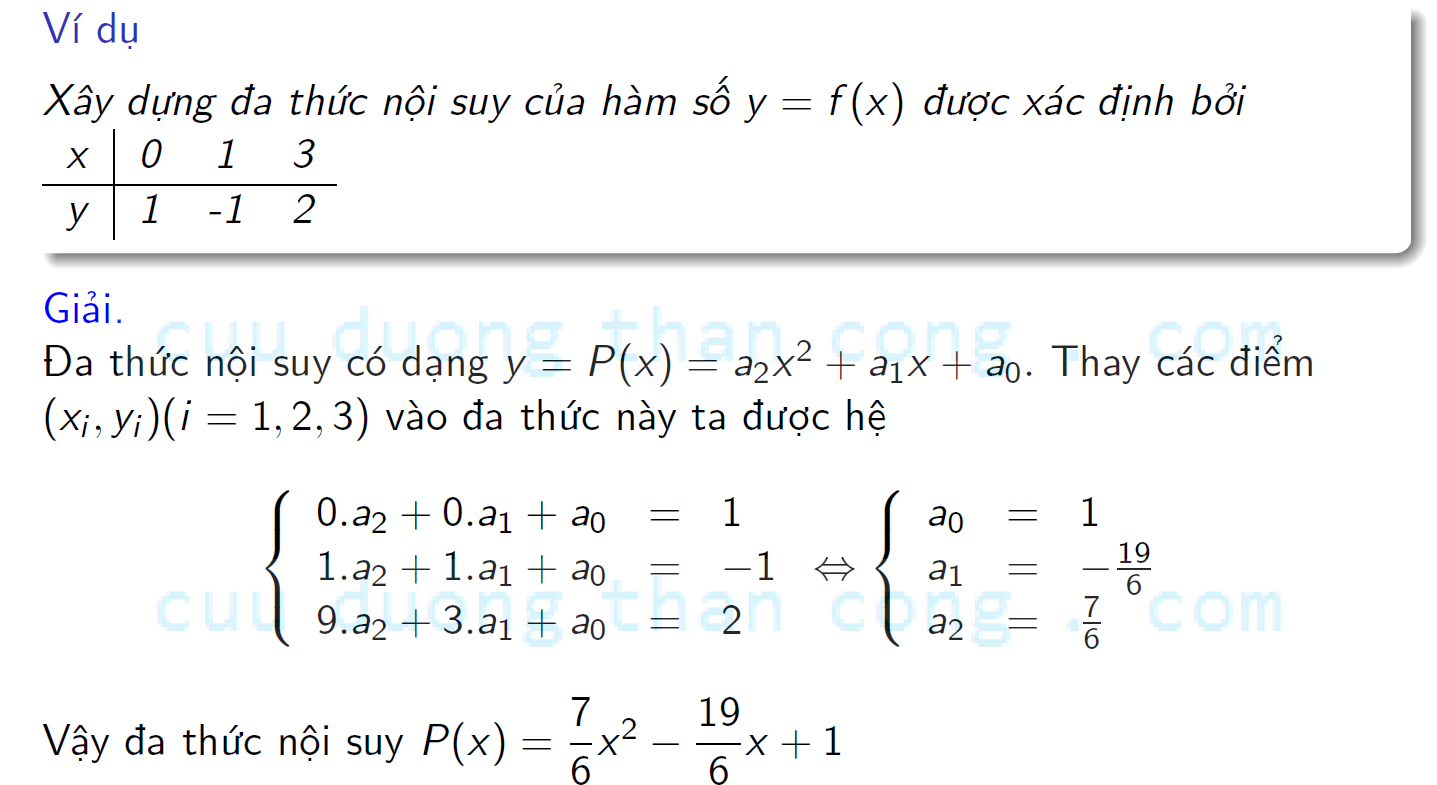
\includegraphics[scale = 0.45]{5.png}
\end{center}
Cho hàm số $y=f(x)$ được xác định như sau: 
\begin{table}[h]
\begin{tabular}{c|ccccc}
$x$ & $x_0$ & $x_1$ & $x_2$ & $\ldots$ & $x_n$ \\ \hline
$y$ & $y_0$ & $y_1$ & $y_2$ & $\ldots$ & $y_n$
\end{tabular}
\end{table}
Ta sẽ xây dựng đa thức nội suy của hàm $f(x)$ trên đoạn $\lbrack x_0,x_n \rbrack, n \geqslant 1$. Đa thức nội suy Larange có dạng như sau $\mathcal{L}_n (x) = \displaystyle \sum_{k=0}^{n} p^k_n (x).y_k$, trong đó
\[
    p^k_n (x) = \frac{(x-x_0)(x-x_1)\ldots(x-x_{k-1})(x-x_{k+1})\ldots (x-x_n)}{(x_k-x_0)(x_k-x_1)\ldots(x_k-x_{k-1})(x_k-x_{k+1})\ldots (x-x_n)}
\]
Larange xây dựng một đa thức bậc n với cơ sở là n đa thức bậc n: $p^k_n (x)$ và $y_k$ là tọa độ tương ứng.\\
\textbf{Chú ý:} $p^k_n (x_k) = 1; p^k_n (x_i) = 0, i \neq k \Rightarrow \mathcal{L}_n (x_k) = y_k$. Đa thức đi qua các điểm $(x_k,y_k)$.
\newpage
\textbf{VD:} Cho bảng số, \begin{table}[h]
    \begin{tabular}{c|ccccc}
    $x$ & $1$ & $1.3$ & $1.7$ & $2$  \\ \hline
    $y$ & $1.82$ & $2.13$ & $3.36$ & $4.7$
    \end{tabular}
    \end{table}
sử dụng đa thức nội suy Larange, tính xấp xỉ giá trị của hàm tại $x=1.44$
\[
    \begin{aligned}
\text{Cách 1: }    L(x) &= 1.82 \times \frac{(x-1.3)(x-1.7)(x-2)}{(1-1.3)(1-1.7)(1-2)} + 2.13 \times \frac{(x-1)(x-1.7)(x-2)}{(1.3-1)(1.3-1.7)(1.3-2)} \\
               &+ 3.36 \times \frac{(x-1)(x-1.3)(x-2)}{(1.7-1)(1.7-1.3)(1.7-2)} + 4.7 \times \frac{(x-1)(x-1.3)(x-1.7)}{(2-1)(2-1.3)(2-1.7)}
    \end{aligned}
\]
\[
    \Rightarrow L(1.44) = 2.4692    
\]
Cách 2:
\begin{table}[h]
    \centering
    \begin{tabular}{c|cccc|c}
    {\color[HTML]{FF0000} $1.44$} & $1$                             & $1.3$                             & $1.7$                             & $2$                             &                                           \\ \hline
    $1$                           & {\color[HTML]{FF0000} $1.44-1$} & $1-1.3$                           & $1-1.7$                           & $1-2$                           & $D_0 = -0.09240$                          \\
    $1.3$                         & $1.3-1$                         & {\color[HTML]{FF0000} $1.44-1.3$} & $1.3-1.7$                         & $1.3-2$                         & $D_1 = 0.01176$                           \\
    $1.7$                         & $1.7-1$                         & $1.7-1.3$                         & {\color[HTML]{FF0000} $1.44-1.7$} & $1.7-2$                         & $D_2 =0.02184 $                           \\
    $2$                           & $2-1$                           & $2-1.3$                           & $2-1.7$                           & {\color[HTML]{FF0000} $1.44-2$} & $D_3 = -0.11760$                          \\ \hline
                                  &                                 &                                   &                                   &                                 & {\color[HTML]{000000} $\omega = 0.00897$}
    \end{tabular}
\end{table}
\[
    y(1.44) = \omega \left( \frac{y_0}{D_0} + \frac{y_1}{D_1} + \frac{y_2}{D_2} + \frac{y_3}{D_3} \right) = 2.4692
\]
\textulc{Note}: $D$ được tính bằng $(1.44-1)\times(1-1.3)\times(1-1.7)\times(1-2)$, $\omega$ được tính bằng $(1.44-1)\times(1.44-1.3)\times(1.44-1.7)\times(1.44-2)$.
\section{Đa thức nội suy Newton.}
\subsection{Tỉ sai phân.}
Cho hàm số $f(x)$ xác định như sau:     \begin{tabular}{c|ccccc}
    $x$ & $x_0$ & $x_1$ & $x_2$ & $\ldots$ & $x_n$ \\ \hline
    $y$ & $y_0$ & $y_1$ & $y_2$ & $\ldots$ & $y_n$ 
    \end{tabular} \text{ trên đoạn $\lbrack a,b \rbrack = \lbrack x_0,x_n \rbrack$}\\   
\DN Trên đoạn $\lbrack x_k, x_{k+1} \rbrack$ ta định nghĩa đại lượng
\[
    f \lbrack x_k, x_{k+1} \rbrack = \frac{y_{k+1} - y_k}{x_{k+1} - x_k} = \frac{y_k - y_{k+1}}{x_k - x_{k+1}} = f\lbrack x_{k+1}, x_k \rbrack
\]
được gọi là tỉ sai phân cấp 1 của hàm trên đoạn $\lbrack x_k, x_{k+1} \rbrack$.\\
Tương tự ta có tỉ sai phân cấp 2 của hàm trên đoạn $\lbrack x_k, x_{k+2} \rbrack$ là 
\[
    f\lbrack x_k, x_{k+1},x_{k+2} \rbrack = \frac{\lbrack x_{k+1}, x_{k+2} \rbrack - f\lbrack x_k, x_{k+1} \rbrack}{x_{k+2} - x_k}
\]
Quy nạp lại ta có tỉ sai phân cấp p của hàm trên đoạn $\lbrack x_k, x_{k+p} \rbrack$ là 
\[
    f\lbrack x_k, x_{k+1},\ldots,x_{k+p} \rbrack = \frac{f\lbrack x_{k+1}, x_{k+2},\ldots,x_{k+p} \rbrack - f\lbrack x_k, x_{k+1},x_{k+p-1} \rbrack}{x_{k+p} - x_k} 
\]
\subsection{Công thức của đa thức nội suy Newton.}
\DN Công thức $\mathcal{N}^{(1)}_n (x)$ được gọi là công thức Newton tiến xuất phát từ điểm nút $x_0$ của hàm số $f(x)$ và $R_n (x)$ được gọi là sai số của đa thức nội suy Newton. Tương tự, ta có thể xây dựng công thức Newton lùi xuất phát từ điểm nút $x_n$ của hàm số $f(x)$ như sau
\[  
    \begin{aligned}
        \mathcal{N}^{(2)}_n (x) &= y_n + f \lbrack x_{n-1},x_n \rbrack (x-x_n) + f\lbrack x_{n-2},x_{n-1},x_n \rbrack(x-x_{n-1})(x-x_n) \\
                                &+ \ldots + f \lbrack x_0,x_1,\ldots,x_n \rbrack (x-x_1)(x-x_2)\ldots(x-x_n)
    \end{aligned}
\]
Do đó tính duy nhất của đa thức nội suy, ta có với cùng 1 bảng số:
\[
    \mathcal{L}_n (x) = \mathcal{N}^{(1)}_n (x) = \mathcal{N}^{(2)}_n (x)    
\]
\begin{center}
    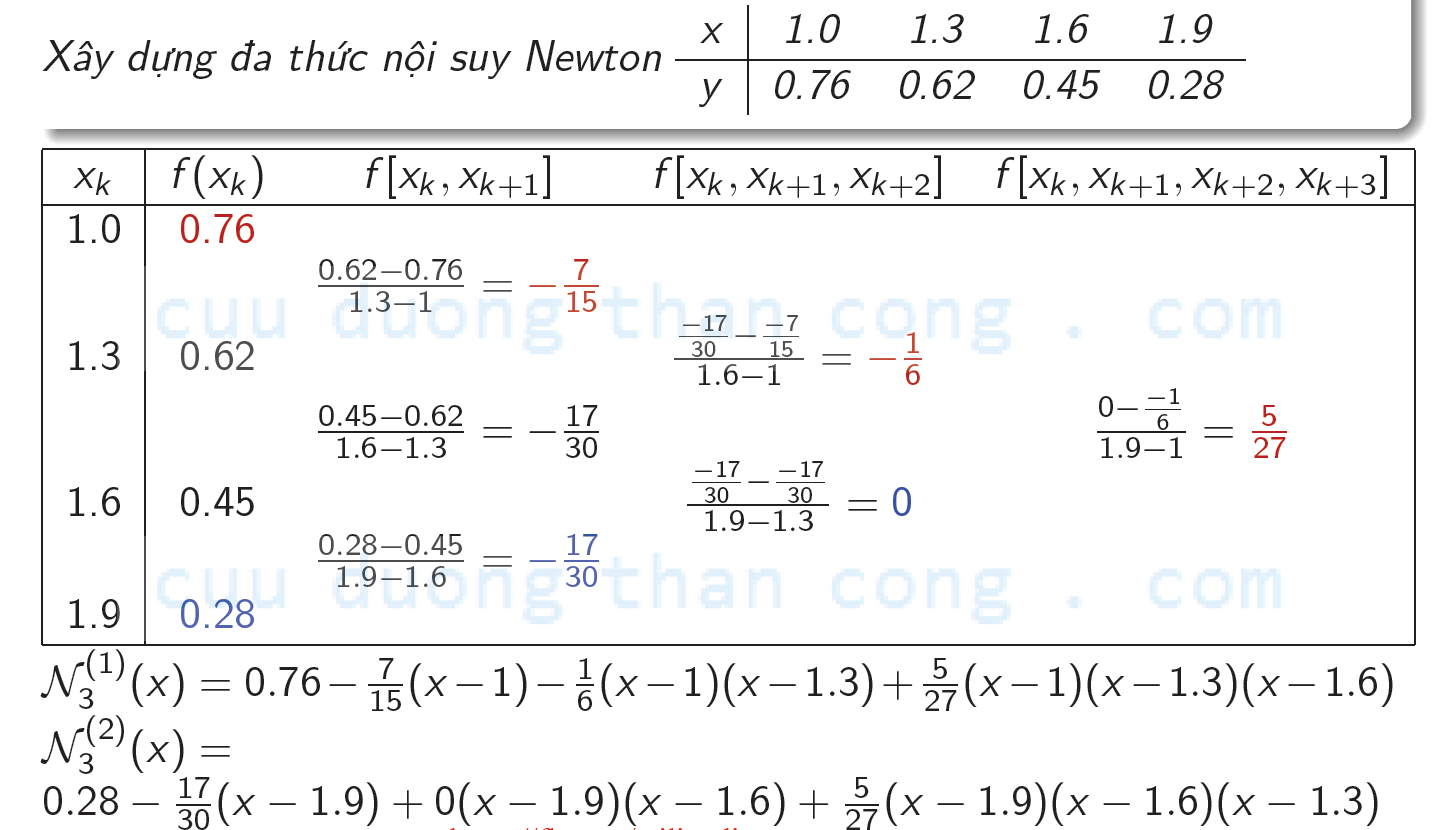
\includegraphics[scale = 0.5]{6.png}
\end{center}
\section{Spline bậc 3.}
\DN Cho bảng số : \begin{tabular}{c|ccccc}
    $x$ & $x_0$ & $x_1$ & $x_2$ & $\ldots$ & $x_n$ \\ \hline
    $y = f(x)$ & $y_0$ & $y_1$ & $y_2$ & $\ldots$ & $y_n$ 
    \end{tabular}, một spline bậc 3 nội suy hàm $f(x)$ trên $\lbrack x_0;x_n \rbrack$ là hàm $g(x)$ thỏa mãn các điều kiện sau:
\begin{enumerate}
    \item $g(x)$ đi qua các điểm nội suy: $g(x_k) = y_k$
    \item $g(x)$ có đạo hàm đến cấp 2 liên tục trên $\lbrack a,b \rbrack$
    \item Trên mỗi đoạn $\lbrack x_k;x_{k+1} \rbrack, k=0,1,\ldots,n-1, g(x) \equiv g(x_k)$ là một đa thức bậc 3.
\end{enumerate}
\subsection{Spline tự nhiên.}
\subsubsection{TH1.} Cho bảng số gồm 3 điểm: \begin{tabular}{c|ccccc}
    $x$ & $x_0$ & $x_1$ & $x_2$ \\ \hline
    $y$ & $y_0$ & $y_1$ & $y_2$  
    \end{tabular}. Xây dựng 2 đa thức bậc 3: 
\[
    \begin{aligned}
        S_0 (x) &= a_0 + b_0(x-x_0) + c_0(x-x_0)^2 + d_0(x-x_0)^3; \thickspace x \in \lbrack x_0,x_1 \rbrack \\
        S_1 (x) &= a_1 + b_1(x-x_1) + c_1(x-x_1)^2 + d_1(x-x_1)^3; \thickspace x \in \lbrack x_1,x_2 \rbrack
    \end{aligned}    
\]
\[
    \begin{cases}
        a_0 = y_0 \\
        a_1 = y_1 \\
        a_2 = y_2 
    \end{cases} \Rightarrow 
    \begin{cases}
        c_0 = 0 \\
        2(h_0 + h_1)c_1 = 3*(\lbrack \thickspace \rbrack_1 - \lbrack \thickspace \rbrack_0) \\
        c_2 = 0
    \end{cases}    
\]
\[
    \text{Chu trình Casio } \underbrace{A - \frac{B}{3}(C+2D)}_{b} : \underbrace{\frac{C - D}{3B}}_{d} \Rightarrow \begin{cases}
        A = \lbrack \thickspace \rbrack_0, B = h_0, C = c_1, D = c_0 \Rightarrow b_0,d_0 \\
        A = \lbrack \thickspace \rbrack_1, B = h_1, C = c_2, D = c_1 \Rightarrow b_1,d_1
    \end{cases}
\]
\subsubsection{TH2.} Cho bảng số gồm 4 điểm: \begin{tabular}{c|ccccc}
    $x$ & $x_0$ & $x_1$ & $x_2$ & $x_3$ \\ \hline
    $y$ & $y_0$ & $y_1$ & $y_2$ & $y_3$
    \end{tabular}. Xây dựng 3 đa thức bậc 3: 
\[
    \begin{aligned}
        S_0 (x) &= a_0 + b_0(x-x_0) + c_0(x-x_0)^2 + d_0(x-x_0)^3; \thickspace x \in \lbrack x_0,x_1 \rbrack \\
        S_1 (x) &= a_1 + b_1(x-x_1) + c_1(x-x_1)^2 + d_1(x-x_1)^3; \thickspace x \in \lbrack x_1,x_2 \rbrack \\
        S_2 (x) &= a_2 + b_2(x-x_2) + c_2(x-x_2)^2 + d_2(x-x_2)^3; \thickspace x \in \lbrack x_2,x_3 \rbrack 
    \end{aligned}    
\]
\[
    \begin{cases}
        a_0 = y_0 \\
        a_1 = y_1 \\
        a_2 = y_2 \\
        a_3 = y_3
    \end{cases} \Rightarrow 
    \begin{cases}
        c_0 = 0 \\
        2(h_0 + h_1)c_1 + h_1c_2 = 3*(\lbrack \thickspace \rbrack_1 - \lbrack \thickspace \rbrack_0) \\
        h_1c_1 +2(h_1 + h_2)c_2 = 3*(\lbrack \thickspace \rbrack_2 - \lbrack \thickspace \rbrack_1) \\
        c_3 = 0
    \end{cases}    
\]
\[
    \text{Chu trình Casio} \underbrace{A - \frac{B}{3}(C+2D)}_{b} : \underbrace{\frac{C - D}{3B}}_{d} \Rightarrow \begin{cases}
        A = \lbrack \thickspace \rbrack_0, B = h_0, C = c_1, D = c_0 \Rightarrow b_0,d_0 \\
        A = \lbrack \thickspace \rbrack_1, B = h_1, C = c_2, D = c_1 \Rightarrow b_1,d_1 \\
        A = \lbrack \thickspace \rbrack_2, B = h_2, C = c_3, D = c_2 \Rightarrow b_2,d_2
    \end{cases}
\]
\textul{Note}: $\lbrack \thickspace \rbrack$ là tỉ sai phân.
\begin{center}
    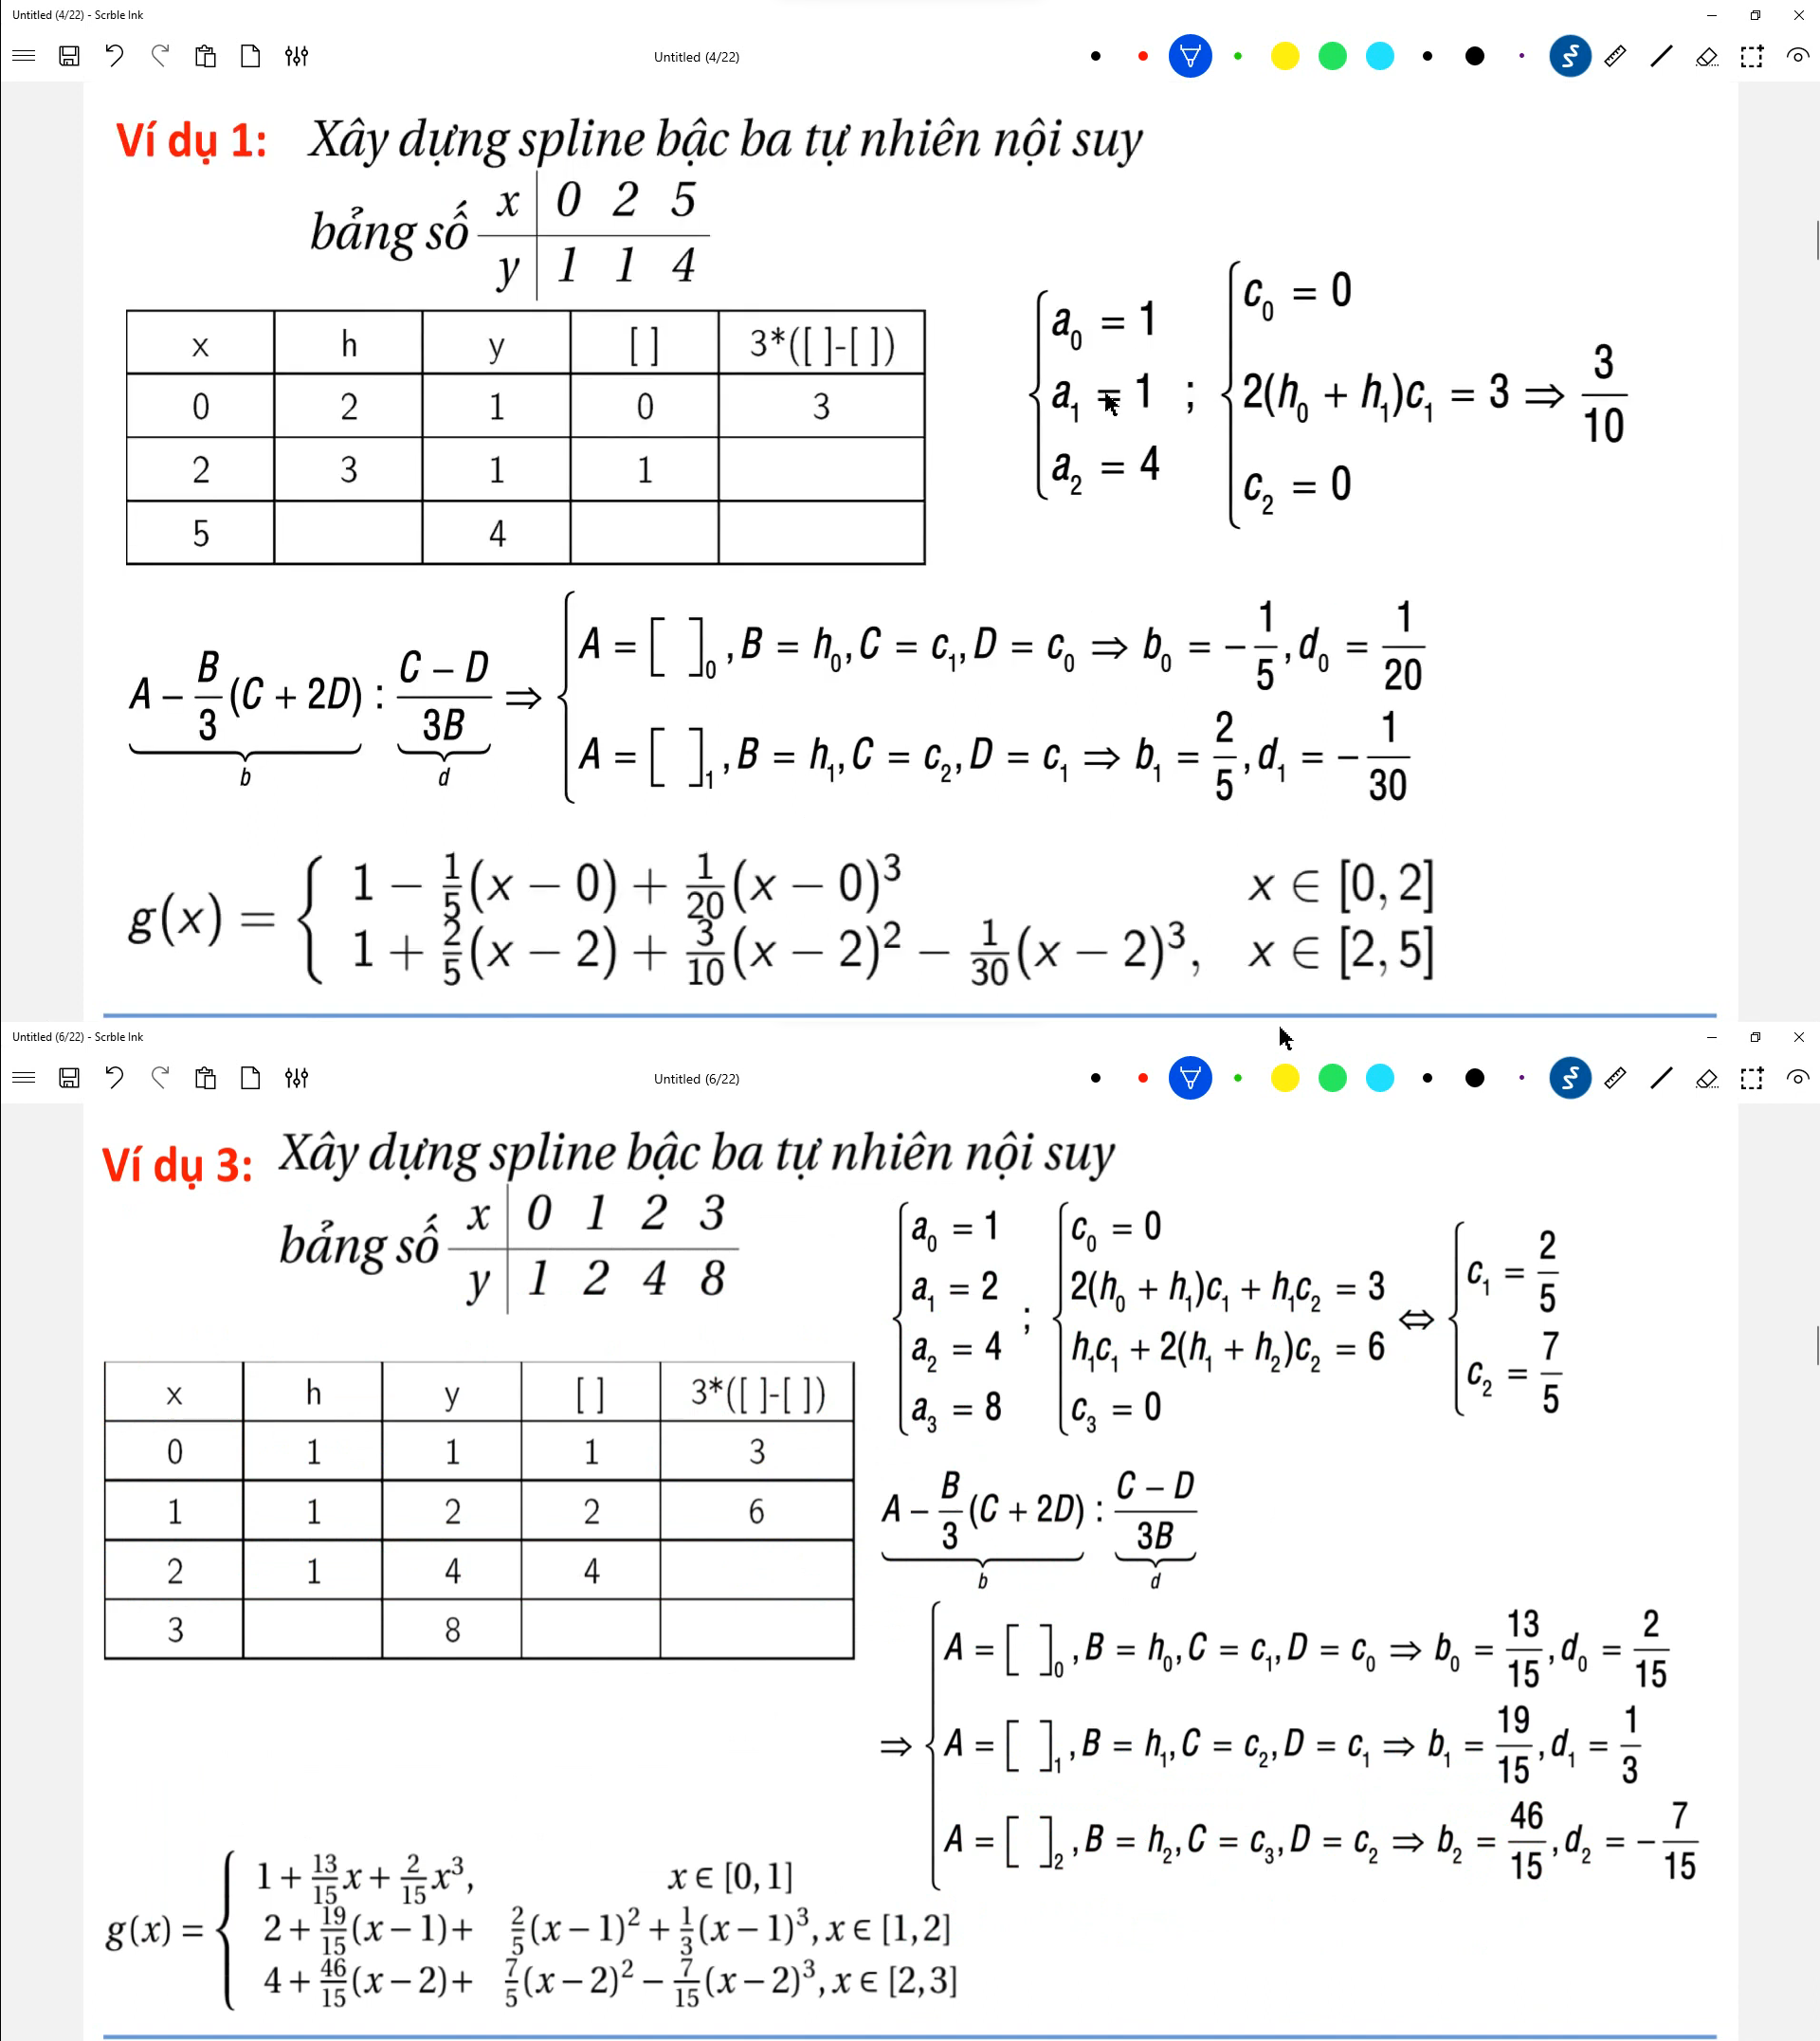
\includegraphics[scale = 0.45]{7.png}
\end{center}
\newpage
\subsection{Spline ràng buộc.}
\subsubsection{TH1.} Cho bảng số gồm 2 điểm: \begin{tabular}{c|ccc}
    $x$ & $x_0$ & $x_1$  \\ \hline
    $y$ & $y_0$ & $y_1$   
    \end{tabular}.
\[
    \begin{pmatrix}
        2h_0 & h_0 \\
        h_0 & 2h_0 
    \end{pmatrix}    \begin{pmatrix}
        c_0 \\
        c_1 
    \end{pmatrix} = \begin{pmatrix}
        \lbrack \thickspace \rbrack_0 \\
        \lbrack \thickspace \rbrack_1 
    \end{pmatrix}
\]
\[
    \text{Chu trình Casio } \underbrace{A - \frac{B}{3}(C+2D)}_{b} : \underbrace{\frac{C - D}{3B}}_{d} \Rightarrow  A = \lbrack \thickspace \rbrack_0, B = h_0, C = c_1, D = c_0 \Rightarrow b_0,d_0 
\]
\subsubsection{TH2.} Cho bảng số gồm 3 diểm: \begin{tabular}{c|ccccc}
    $x$ & $x_0$ & $x_1$ & $x_2$ \\ \hline
    $y$ & $y_0$ & $y_1$ & $y_2$  
    \end{tabular}.
\[
    \begin{pmatrix}
        2h_0 & h_0 & 0 \\
        h_0 & 2(h_0 + h_1) & h_1 \\
        0 & h_1 & 2h_1 
        \end{pmatrix}   \begin{pmatrix}
            c_0 \\
            c_1 \\ 
            c_2
        \end{pmatrix}  = \begin{pmatrix}
            \lbrack \thickspace \rbrack_0 \\
            \lbrack \thickspace \rbrack_1 \\ 
            \lbrack \thickspace \rbrack_2
        \end{pmatrix}  
\]
\[
    \text{Chu trình Casio} \underbrace{A - \frac{B}{3}(C+2D)}_{b} : \underbrace{\frac{C - D}{3B}}_{d} \Rightarrow \begin{cases}
        A = \lbrack \thickspace \rbrack_0, B = h_0, C = c_1, D = c_0 \Rightarrow b_0,d_0 \\
        A = \lbrack \thickspace \rbrack_1, B = h_1, C = c_2, D = c_1 \Rightarrow b_1,d_1
    \end{cases}
\]
\section{Phương pháp bình phương bé nhất (Xấp xỉ hàm thực nghiệm).}
\textbf{TH1. $f(x)=A+Bx$}, khi đó
\[
    g(A,B) = \sum_{k=1}^{n} (A+Bx_k - y_k)^2  
\]
Bài toán quy về việc tìm cực tiểu của hàm 2 biến $g(A,B)$. Tọa độ điểm dừng của hàm được xác định bởi hệ phương trình: 
\[
    \begin{cases}
        nA + \left( \displaystyle \sum_{k=1}^{n} x_k \right) B = \displaystyle \sum_{k=1}^{n} y_k \\
        \left( \displaystyle \sum_{k=1}^{n} x_k \right) A + \left( \displaystyle \sum_{k=1}^{n} x^2_k \right) B = \displaystyle \sum_{k=1}^{n} x_k y_k
    \end{cases}    
\]
\textbf{TH2. $f(x) = A + Bx + Cx^2$}, khi đó
\[
    g(A,B,C) = \sum_{k=1}^{n} (A+Bx_k + Cx^2_k- y_k)^2  
\]
Bài toán quy về việc tìm cực tiểu của hàm 3 biến $g(A,B,C)$. Tọa độ điểm dừng của hàm được xác định bởi hệ phương trình: 
\[
    \begin{cases}
        nA + \left( \displaystyle \sum_{k=1}^{n} x_k \right) B + \left( \displaystyle \sum_{k=1}^{n} x^2_k \right) C= \displaystyle \sum_{k=1}^{n} y_k \\
        \left( \displaystyle \sum_{k=1}^{n} x_k \right) A + \left( \displaystyle \sum_{k=1}^{n} x^2_k \right) B + \left( \displaystyle \sum_{k=1}^{n} x^3_k \right) C= \displaystyle \sum_{k=1}^{n} x_k y_k \\
        \left( \displaystyle \sum_{k=1}^{n} x^2_k \right) A + \left( \displaystyle \sum_{k=1}^{n} x^3_k \right) B + \left( \displaystyle \sum_{k=1}^{n} x^4_k \right) C= \displaystyle \sum_{k=1}^{n} x^2_k y_k
    \end{cases}      
\]
\textbf{TH3. $f(x) = Ag(x) + Bh(x)$}, khi đó
\[
    g(A,B) = \sum_{k=1}^{n} (Ag(x_k) + Bh(x_k) - y_k)^2  
\]
Bài toán quy về việc tìm cực tiểu của hàm 2 biến $g(A,B)$. Tọa độ điểm dừng của hàm được xác định bởi hệ phương trình: 
\[
    \begin{cases}
        \left( \displaystyle \sum_{k=1}^{n} g^2(x_k) \right) A + \left( \displaystyle \sum_{k=1}^{n} g(x_k)h(x_k) \right) B = \displaystyle \sum_{k=1}^{n} g(x_k)y_k \\
        \left( \displaystyle \sum_{k=1}^{n} g(x_k)h(x_k) \right) A + \left( \displaystyle \sum_{k=1}^{n} h^2(x_k) \right) B = \displaystyle \sum_{k=1}^{n} h(x_k)y_k \\
    \end{cases}  
\]
\newpage
\chapter{ĐẠO HÀM VÀ TÍCH PHÂN}
\section{Tính gần đúng đạo hàm.}
Công thức sai phân tiến: 
\[
    f'(x_0) \approx \frac{-3f(x_0) + 4f(x_0 + h) - f(x_0 + 2h)}{2h}    
\]

Công thức sai phân lùi:
\[
    f'(x_0) \approx \frac{f(x_0-2h) + 4f(x_0 - h) + 3f(x_0)}{2h}          
\]

Công thức sai phân hướng tâm:
\[
    f'(x_0) \approx \frac{f(x_0 + h) - f(x_0 - h) }{2h}; f''(x_0) \approx \frac{f(x_0 + h) -2f(x_0) + f(x_0 - h)}{h^2}    
\]
\section{Tính gần đúng tích phân xác định.}
\subsection{Công thức hình thang mở rộng:}
\[
    \int_{a}^{b} f(x) dx \approx \frac{h}{2} (y_0 + 2y_1 + 2y_2 + \ldots + 2y_{n-1} + y_n), \quad \text{với: } x_0 = a, x_k = x_0 + h.k \text{ và } y_k = f(x_k).
\]

Sai số hình thang mở rộng:
\[
    \Delta I = \frac{M_2 (b-a)^3}{12n^2} = \frac{\displaystyle\max_{x \in \lbrack a;b \rbrack} |f''(x)| (b-a)^3}{12n^2}    
\]
\subsection{Công thức Simpson:}
\[
    \int_{a}^{b} f(x) dx = \frac{h}{3}(f(a) + f(x_1) + f(b)), \quad \text{với } x_1 = a + h, h = \frac{b-a}{2}
\]

Công thức Simpson mở rộng: 
\[
    \int_{a}^{b} f(x) dx \approx \frac{h}{3}(y_0 + 4y_1 + 2y_2 + 4y_3 + \ldots + 2y_{n-1} + y_n)    
\]

Sai số Simpson mở rộng: 
\[
    \Delta I = \frac{n}{2}.\frac{M_4h^5}{90} = \frac{\displaystyle\max_{x \in \lbrack a;b \rbrack} |f^{(4)}(x)|  (b-a)^5}{180n^4}  
\]
\subsection{Cầu phương Gauss: (bỏ)}
Công thức cầu phương Gauss bậc hai:
\[
    \int_{-1}^{1} f(x) dx \approx f \left( -\sqrt{\frac{1}{3}} \right) + f \left( \sqrt{\frac{1}{3}} \right)  
\]

Công thức cầu phương Gauss bậc ba:
\[
    \int_{-1}^{1} f(x) dx \approx \frac{5}{9} f \left( -\sqrt{\frac{3}{5}} \right) + \frac{8}{9}f(0) + \frac{5}{9} f \left( \sqrt{\frac{3}{5}} \right)  
\]

Chú ý: Khi tính $I = \displaystyle \int_{a}^{b} f(x)dx$ theo cầu phương Gauss. Ta đặt
\[
    x = \frac{b-a}{2}t  + \frac{b+a}{2} \rightarrow dx = dt    
\]
\[
    \Rightarrow I = \frac{b-a}{2} \displaystyle \int_{-1}^{1} f \left( \frac{b-a}{2}t  + \frac{b+a}{2} \right) dt 
\]
Nhân $\dfrac{b-a}{2}$ vào 2 công thức bậc 3 và 2.

\begin{center}
    \includegraphics*[scale = 0.28]{8.png}
\end{center}
\newpage
\chapter{PHƯƠNG TRÌNH VI PHÂN}
Điều kiện ban đầu của bài toán:
\[
    \begin{cases}
        y' = f(x,y), \quad a \leqslant x \leqslant b \\
        y(x_0) = y_0
    \end{cases}    
\]
\section{Phương pháp Euler.}
\[
    y_1 = y_0 + hf(x_0,y_0)  
\]
\section{Phương pháp Euler cải tiến.}
\[
    A = hf(X,Y)    
\]
\[
    X = X + h    
\]
\[
    B = hf(X,Y+A)    
\]
\[
    Y = Y + \frac{A+B}{2}    
\]
\section{Phương pháp Runge-Kutta.}
\[
    y_1 = y_0 + \frac{A + 2B + 2C + D}{6}    
\]
\[
    \begin{cases}
        A = hf(x_0,y_0) \\
        B = hf(x_0 + \dfrac{h}{2}, y_0 + \dfrac{A}{2}) \\
        C = hf(x_0 + \dfrac{h}{2}, y_0 + \dfrac{B}{2}) \\
        D = hf(x_0 + h, y_0 + C)
    \end{cases}    
\]
\section{Hệ phương trình vi phân.}
Xét hệ:
\[
    \begin{cases}
        y' = F(x,y,z) \\
        z' = G(x,y,z) \\
        y(x_0) = y_0, z(x_0) = z_0
    \end{cases}    
\]
\subsection{Euler.}
\[
    A = Y + hF(X,Y,Z) \thickspace : \thickspace B = Z + hG(X,Y,Z) \thickspace : \thickspace Y = A : Z = B \thickspace : \thickspace X = X + h 
\]
\[
    \begin{cases}
        Y = y_0, Z = z_0 \\
        A = y_1, B = z_1
    \end{cases}
\]
\subsection{Euler cải tiến.}
\[
    A = hF(X,Y,Z)  :  B = hG(X,Y,Z)  :  X = X + h  :  C = hF(X,Y+A,Z+B) :
\]
\[
    D = hG(X,Y+A,Z+B) : Y = Y + \frac{A+C}{2} : Z = Z + \frac{B+D}{2}
\]
\section{Phương trình vi phân cấp hai.}
\begin{itemize}
    \item Cách 1: Đưa về hệ ptvp, dùng pp Euler hoặc Euler cải tiến.
    \item Cách 2: Dùng phương pháp sai phân hữu hạn.
\end{itemize}
\[
    p(x).y''(x) + q(x).y'(x) + r(x).y(x) = f(x)    
\]
\[
  \text{Cho } y_0, y_3 \longrightarrow  
    \begin{cases}
        \left( r - \dfrac{2p}{h^2} \right)y_1 + \left(\dfrac{p}{h^2} + \dfrac{q}{2h} \right)y_2 = f(x) - \left(\dfrac{p}{h^2} -\dfrac{q}{2h} \right)y_0 \text{ (tính tại } x_1) \\
        \left(\dfrac{p}{h^2} - \dfrac{q}{2h} \right)y_1 + \left( r - \dfrac{2p}{h^2} \right)y_2 = f(x) - \left(\dfrac{p}{h^2} + \dfrac{q}{2h} \right)y_3 \text{ (tính tại } x_2)
    \end{cases}    
\]
\[
    \text{Cho } y_0, y_4 \longrightarrow  
    \begin{cases}
        \left( r - \dfrac{2p}{h^2} \right)y_1 + \left(\dfrac{p}{h^2} + \dfrac{q}{2h} \right)y_2 + 0y_3 = f(x) - \left(\dfrac{p}{h^2} - \dfrac{q}{2h} \right)y_0 \text{ (tính tại } x_1) \\
        \left(\dfrac{p}{h^2} - \dfrac{q}{2h} \right)y_1 + \left( r - \dfrac{2p}{h^2} \right)y_2 + \left(\dfrac{p}{h^2} + \dfrac{q}{2h} \right)y_3 = f(x) \text{ (tính tại } x_2) \\
        0y_1 + \left(\dfrac{p}{h^2} - \dfrac{q}{2h} \right)y_2 + \left( r - \dfrac{2p}{h^2} \right)y_3 = f(x) - \left(\dfrac{p}{h^2} + \dfrac{q}{2h} \right)y_4 \text{ (tính tại } x_3)
    \end{cases}
\]
\end{document}